\documentclass{article}
\usepackage[a4paper, hmargin={2.8cm, 2.8cm}, vmargin={2.5cm, 2.5cm}]{geometry}
%%%%%%%%%%%%%%%%%%%%%%%%%%%%%%%%%%%%%%%%%%%%%%%%%%%%%%%%%%%%%%%%%%%%%%%%%%%%%%%%

%%%%%%%%%%%%%%%%%%%%%%%%%%%%%%%%%%%%%%%%%%%%%%%%%%%%%%%%%%%%%%%%%%%%%%%%%%%%%%%%
\usepackage[utf8]{inputenc}
\usepackage[T1]{fontenc}
%%%%%%%%%%%%%%%%%%%%%%%%%%%%%%%%%%%%%%%%%%%%%%%%%%%%%%%%%%%%%%%%%%%%%%%%%%%%%%%%


%%%%%%%%%%%%%%%%%%%%%%%%%%%%%%%%%%%%%%%%%%%%%%%%%%%%%%%%%%%%%%%%%%%%%%%%%%%%%%%%
\usepackage{mathtools}
\usepackage{amsthm}
\usepackage{amssymb}
\usepackage{csvsimple}
\usepackage{subcaption}
\usepackage{url}
\usepackage{tikz}
\usepackage{pgfplots}
%%%%%%%%%%%%%%%%%%%%%%%%%%%%%%%%%%%%%%%%%%%%%%%%%%%%%%%%%%%%%%%%%%%%%%%%%%%%%%%%


%%%%%%%%%%%%%%%%%%%%%%%%%%%%%%%%%%%%%%%%%%%%%%%%%%%%%%%%%%%%%%%%%%%%%%%%%%%%%%%%
\usepackage{fancyhdr}
\usepackage{graphicx}
\usepackage{parskip}
\usepackage{listings}
\usepackage{enumitem}
\usepackage{titlesec}
\usepackage[lastpage,user]{zref}
\usepackage{caption}
\usepackage{scrextend}
% \usepackage[outputdir=./.latex-out]{minted} % TODO slet hvis du ikke bruger minted
\usepackage{listings}
\usepackage{blindtext}
%%%%%%%%%%%%%%%%%%%%%%%%%%%%%%%%%%%%%%%%%%%%%%%%%%%%%%%%%%%%%%%%%%%%%%%%%%%%%%%%
\newcommand{\python}[1] {
  \mintinline{python}{#1}
}
\newcommand{\tex}[1] {
  \mintinline{latex}{#1}
}
\pagestyle{fancy}
%%%%%%%%%%%%%%%%%%%%%%%%%%%%%%%%%%%%%%%%%%%%%%%%%%%%%%%%%%%%%%%%%%%%%%%%%%%%%%%%
%%%%%%%%%%%%%%%%%%%%%%%%%%%%%%%%%%%%%%%%%%%%%%%%%%%%%%%%%%%%%%%%%%%%%%%%%%%%%%%%
\lhead{\LaTeX webinar} % TODO indsæt venstre sidehoved
\rhead{Study Now} % TODO indsæt højre sidehoved
\cfoot{\thepage\ of \zpageref{LastPage}}
\newtheorem*{prp}{Propostion}
\setlist{nolistsep}
%%%%%%%%%%%%%%%%%%%%%%%%%%%%%%%%%%%%%%%%%%%%%%%%%%%%%%%%%%%%%%%%%%%%%%%%%%%%

%%%%%%%%%%%%%%%%%%%%%%%%%%%%%%%%%%%%%%%%%%%%%%%%%%%%%%%%%%%%%%%%%%%%%%%%%%%%
\title{
  \vspace{13em}
  \large{Study Now} \\
  \Large{\LaTeX webinar} \\
}

\author{
  Benjamin Rotendahl --- Benjamin@Rotendahl.dk
}

\date{
  \vspace{22em}
  \today
}
%%%%%%%%%%%%%%%%%%%%%%%%%%%%%%%%%%%%%%%%%%%%%%%%%%%%%%%%%%%%%%%%%%%%%%%%%%%%


\begin{document}
\maketitle

\newpage
\tableofcontents

\newpage

\section{Introduktion til \LaTeX}
This document is as a \emph{cheat sheet}. It covers how to setup a \LaTeX{}
document and showcases the most common \LaTeX{} commands and functions.
You have both the pdf and source code such that you can add other cool commands
you find on your journey. Vil du se en sej figur, så kig i section~\ref{sec:latex_to_pdf}

We have that a partial derivative is given by
\begin{flalign}
	\frac{\partial f}{\partial x} & = 4x + 4y \\
	\frac{\partial f}{\partial y} & = 6y + 4x
\end{flalign}

\section{Introduction}


\section{\LaTeX{} background}
Before diving into the syntax of \LaTeX{} you should know a bit about the
process of writing \LaTeX{} documents. \LaTeX{} is a typesetting program and
language. The main advantage of \LaTeX{} is its ability to typeset math, code
and other scientific/technical figures. \LaTeX{} in an extension of TeX, which
released by Donald Knuth in the year 1981.

\subsection{From source code to PDF}\label{sec:local}
\LaTeX{} is not a word processor, but a language and compiler which given a
file containing source code, written in an \emph{editor}, creates a PDF.
as mentiond in section~\ref{sec:local}


An editor for local use, could be \emph{Visual studio code}\cite{vscode}, it
can be used to write any programming/markup language. Support for languages
comes through packages that extends its functionality, there exists packages
for most languages such as python, javascript and \LaTeX{}\cite{latexPackage}.

After the editor has saved the source code, it must be passed to the compiler.
This can be setup to happen automatically on save. There are different versions
of the compiler, they differ in the amount of packages and features they come
with.  ``The latex project TeX''\cite{texLive} has links to various distributions
for the most common operating systems.
With an editor and compiler installed you are ready to write \LaTeX{}.
The processes is illustrated in figure~\ref{fig:compile}.
\subsection{Fra kildekode til PDF}\label{sec:latex_to_pdf}

\section{Matematik i \LaTeX}
After the editor has saved the source code, it must be passed to the compiler.
This can be setup to happen automatically on save. There are different versions
of the compiler, they differ in the amount of packages and features they come
with.  ``The latex project TeX''\cite{texLive} has links to various distributions
for the most common operating systems.
With an editor and compiler installed you are ready to write \LaTeX{}.

Der er mange cirkelkonstanter den bedste er \(\pi = 2 \cdot \tau\) de er seje
givet et vilkårligt \(x\) som er mindre end \(x < n\) så kanm vi.
\[
\pi = \frac{1}{2} \tau
\]

\begin{quote}
	Tau er altså bedre end pi sagde min forlæser se bare på ligning~\ref{eq:tau}
\end{quote}


\begin{equation}\label{eq:tau}
	\pi = \frac{1}{2} \tau
\end{equation}



\begin{equation*}
	2\pi =  \tau
\end{equation*}

hej med jer!
\begin{flalign*}
	f(x,y)                        & = 2x^2 + 3y^2 + 4xy \\
	\frac{\partial f}{\partial x} & = 4x + 4y           \\
	\frac{\partial f}{\partial y} & = 6y + 4x
\end{flalign*}
Der er mange cirkelkonstanter den bedste er \(\pi = 2 \cdot \tau\) de er seje
givet et vilkårligt \(x\) som er mindre end \(x < n\) så kanm vi.
Det er en normalfordeling givet ved
\[
f(x_{1}, x_2, \dots, x_n) = \int_{i=0}^{n} x_i \,dx
\]


\subsection{Figure}
Vi skal have noget grafik!
\begin{figure}
\centering
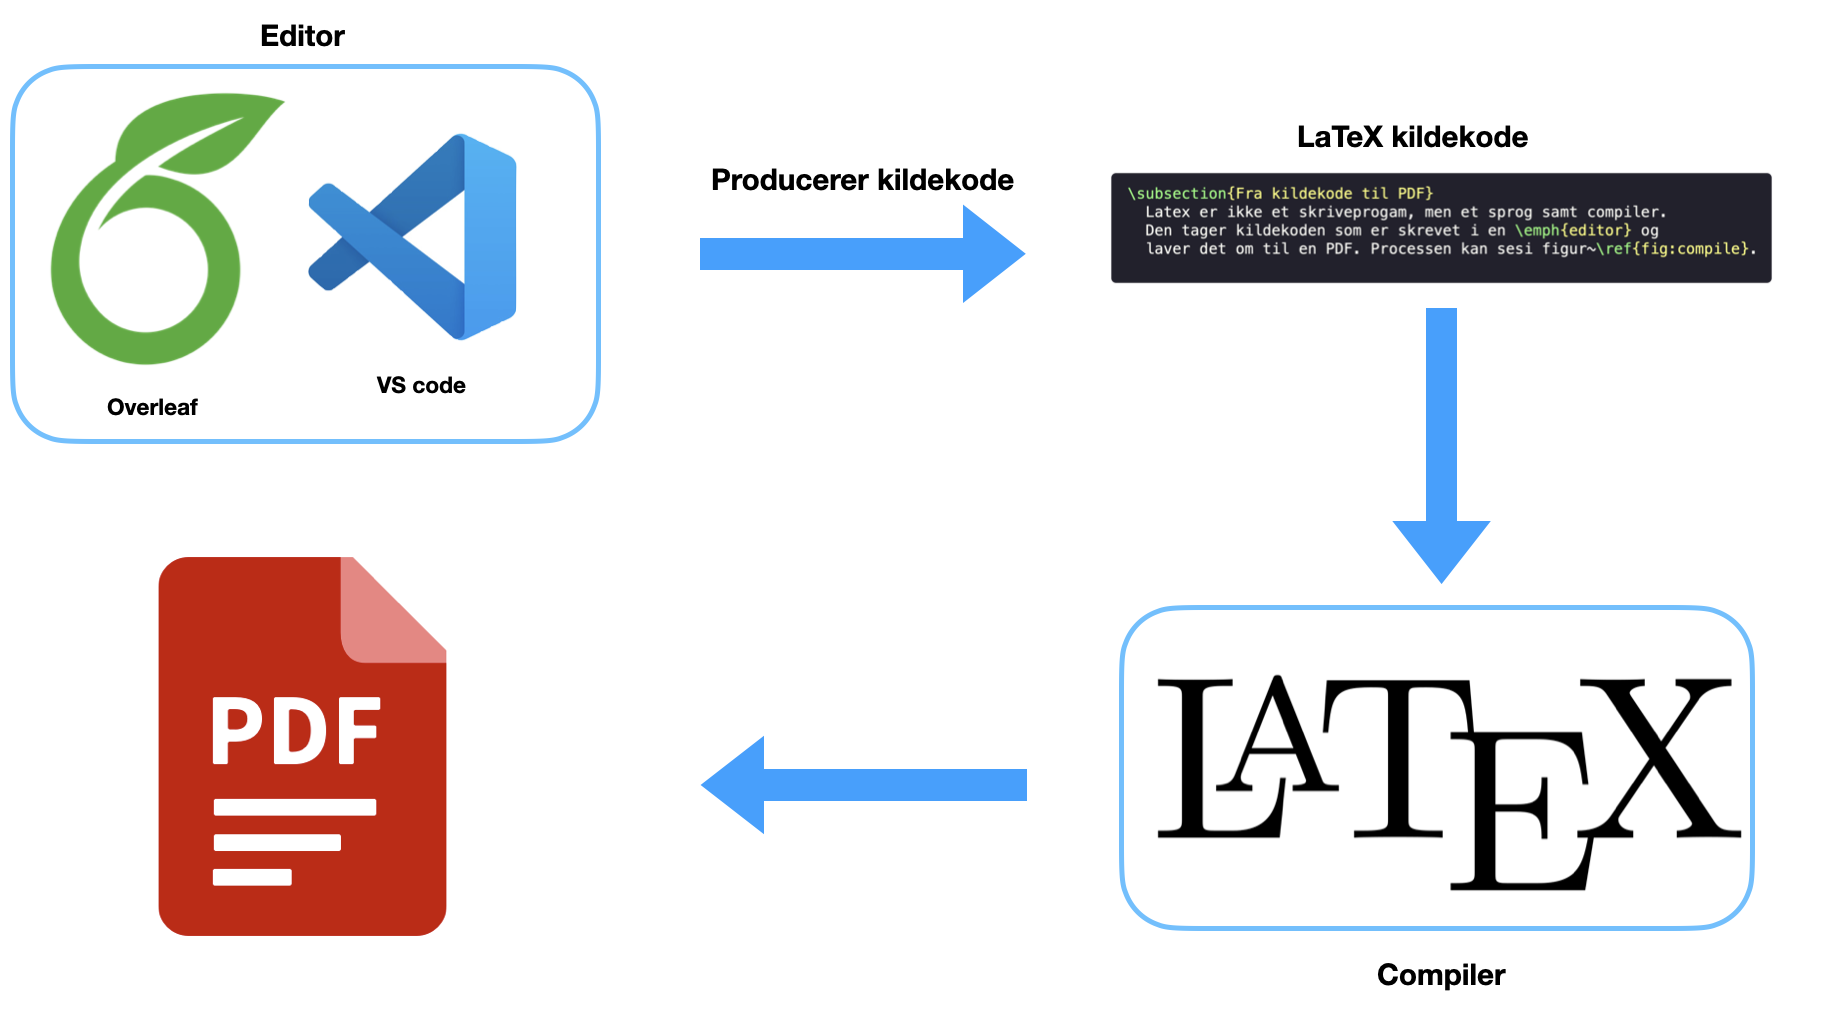
\includegraphics[width=0.8\linewidth]{assets/compile.png}
\caption{The process of compiling \LaTeX{} source code to PDF}
\label{fig:compile}
\end{figure}

Der er mange cirkelkonstanteor den bedste er \(\pi = 2 \cdot \tau\) de er seje
givet et vilkårligt \(x\) som er mindre end \(x < n\) så kanm vio.
as shown in\cite{latexPackage}


\newpage
\appendix
\bibliography{assets/references}{}
\bibliographystyle{plain}

\begin{table}
	\centering
	\begin{tabular}{l | c | c }
		Navn     & Studie   & Semester \\ \hline
		Benjamin & Datalogi & 3        \\ \hline
		Mads     & Historie & 5        \\ \hline
		Ida      & Biologi  & 6        \\ \hline
	\end{tabular}
	\caption{En tabel med studerende}
	\label{tab:studerende}
\end{table}

En auto tabel:
\begin{table}
	\centering
	\csvautotabular{assets/dices.csv}
	\caption{En auto tabel}
	\label{tab:studerende}
\end{table}

\newpage
\appendix
\bibliography{../assets/references}{}
\bibliographystyle{plain}

\newpage
\subsection{\LaTeX{} tankegang \& syntax}

\subsubsection{Kommando syntax}

\subsection{Referencemateriale og problemløsning}




\subsection{Matematikoperationer og notationer}

\subsection{Matricer og vektorer}

\section{Figurerer}

\section{Lister}

\section{Tabeller}


\section{Kodetekst}

\section{Referencer}


\end{document}

